\section{Experiments}

\subsection{Z-score Versus Activation-score}

Z-score is one of the most used methods in linguistic statistics. It compares the observed frequency of a word with the frequency expected in the case of a "normal" distribution. This calculation readily gives, for example, the most specific vocabulary of a given author in a contrastive corpus. The highest z-scores are the most specific words in this case. This is a simple but strong method for analyzing features of text. It can also be used to classify word sequences according to the global z-score (sum of the score) in the sequence. The mean accuracy of this method on our data set is around 85\%, which confirms z-score is in fact meaningful on contrastive data. On the other hand, most of the time deep learning attains greater than 90\% accuracy in text classification. This means that the training methods can learn also on their own some of the linguistic specificities useful in distinguishing between classes of text or authors. We've seen in work on images that thi is the role of convolution. It learns an abstraction of the data to make classification easier. The question is: what is the nature of this abstraction on text? We will see now that deep learning detects automatically words with hight z-score but apparently this is not the only linguistic structure detected.

\begin{figure}[h]
\begin{center}
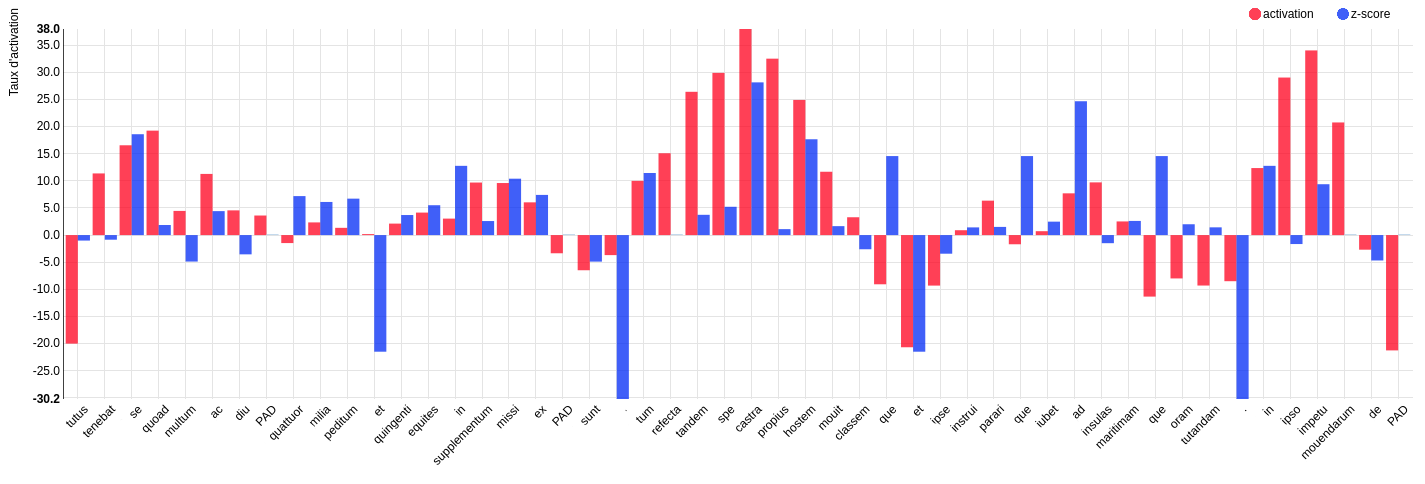
\includegraphics[width=7.5cm]{img/z-score_activations.png}
\caption{Z-score versus Activation-score}
\label{comparision}
\end{center}
\end{figure}

The Figure \ref{comparision} shows us a comparison between z-score and activation-score on a sequence extract form our latin corpora (Livy Book XXIII Chap. 26). Here it's an example of specific word use by Livy\footnote{Titus Livius Patavinus -- (64 or 59 BC - AD 12 or 17) -- was a Roman historian.}. As we can see, when the z-score is the highest there is a sort of activation spike around the word \textit{castra}. However, this is not always the case: for example small words as \textit{que}, \textit{ad} and \textit{et} are also high in z-score but they do not activate the network at the same level. We saw in (reference ****) that deeplearning is more sensitive to long words, but we can see also on Figure \ref{comparision} that words like \textit{tenebat}, \textit{multum} or \textit{propius} are totally uncorrelated. The Pearson\footnote{Pearson correlation coefficient measures the linear relationship between two datasets. It has a value between $+1$ and $-1$, where $1$ is total positive linear correlation, $0$ is no linear correlation, and $-1$ is total negative} correlation coefficient tells us that in this sequence there is no correlation between z-score and activation-score (with a Pearson of 0.38). This example is one of the most correlated examples of our dataset, thus deep learning seems to learn more than a simple z-score.

In order to understand what the real linguistic marks found by deeplearning are (the convolution layer), we did several tests on different languages and our model seems to have the same behavior in all of them. We used a French web-platform called Hyperbase\footnote{Hyperbase is an on-line (\textit{http://hyperbase.unice.fr}) linguistic toolbox, which allows the creation of databases from textual corpus and the performing of analysis and calculations such z-score, cooccurrences, PCA, K-Means distance, ... } to perform all the linguistic statistics tests. 

\subsection{Dataset: English}

The first dataset we used for our experiments is the well known IMDB Movie review corpus for sentiment classification. It consists of 25,000 reviews labeled by positive or negative sentiment with around 230,000 words. With the default methods given by Hyperbase, we can easily show the specific vocabulary of each class (positive/negative), according to the z-score. There are for example the words \textit{too}, \textit{bad}, \textit{no} or \textit{boring} as most indicitive of negative sentiment, and the words \textit{and}, \textit{performance}, \textit{powerful} or \textit{best} for positive. 
Is it enough to detect automatically if a new review is positive or not? Let's see an example excerpted from a review from December 2017 (not in the training set) on the last American blockbuster:

\begin{quote}
\textit{[...] \textcolor{red}{\textbf{i enjoyed three moments}} in the film in total , \textcolor{red}{\textbf{and if i am being honest and}} the person \textcolor{red}{\textbf{next to me fell asleep}} in the middle and started snoring during the slow space chasescenes . \textcolor{red}{\textbf{the story failed to}} draw me in and entertain \textcolor{red}{\textbf{me the way}} [...]} 
\end{quote}%%%verify this citation

In general the z-score is enough to predict the class of this kind of comment. But in this case, deeplearning seems to do better, but why? If we sum all the z-scores (for negative and positive), the positive class obtains a greater score than the negative. The words \textit{film}, \textit{and}, \textit{honest} and \textit{entertain} -- with scores 5.38, 12.23, 4 and 2.4 -- make this example positive. Deep learning has activated different parts of this sequence (as we show in bold/red in the exemple). If we take the sub-sequence \textit{and if i am being honest and}, there are two occurences of \textit{and} but the first one is followed by \textit{if} and Hyperbase give us 0.84 for \textit{and if} as a negative class. This is far from the 12.23 in the positive. And if we go further, we can do a co-occurrence analysis on \textit{and if} on the training set. As we see on Figure \ref{and_if}, one of most specific adjectives\footnote{With Hyperbase we can focus on different part of speech.} associated with \textit{and if} is \textit{honest}. Exactly what we found in our example. 

\begin{figure}[h]
\begin{center}
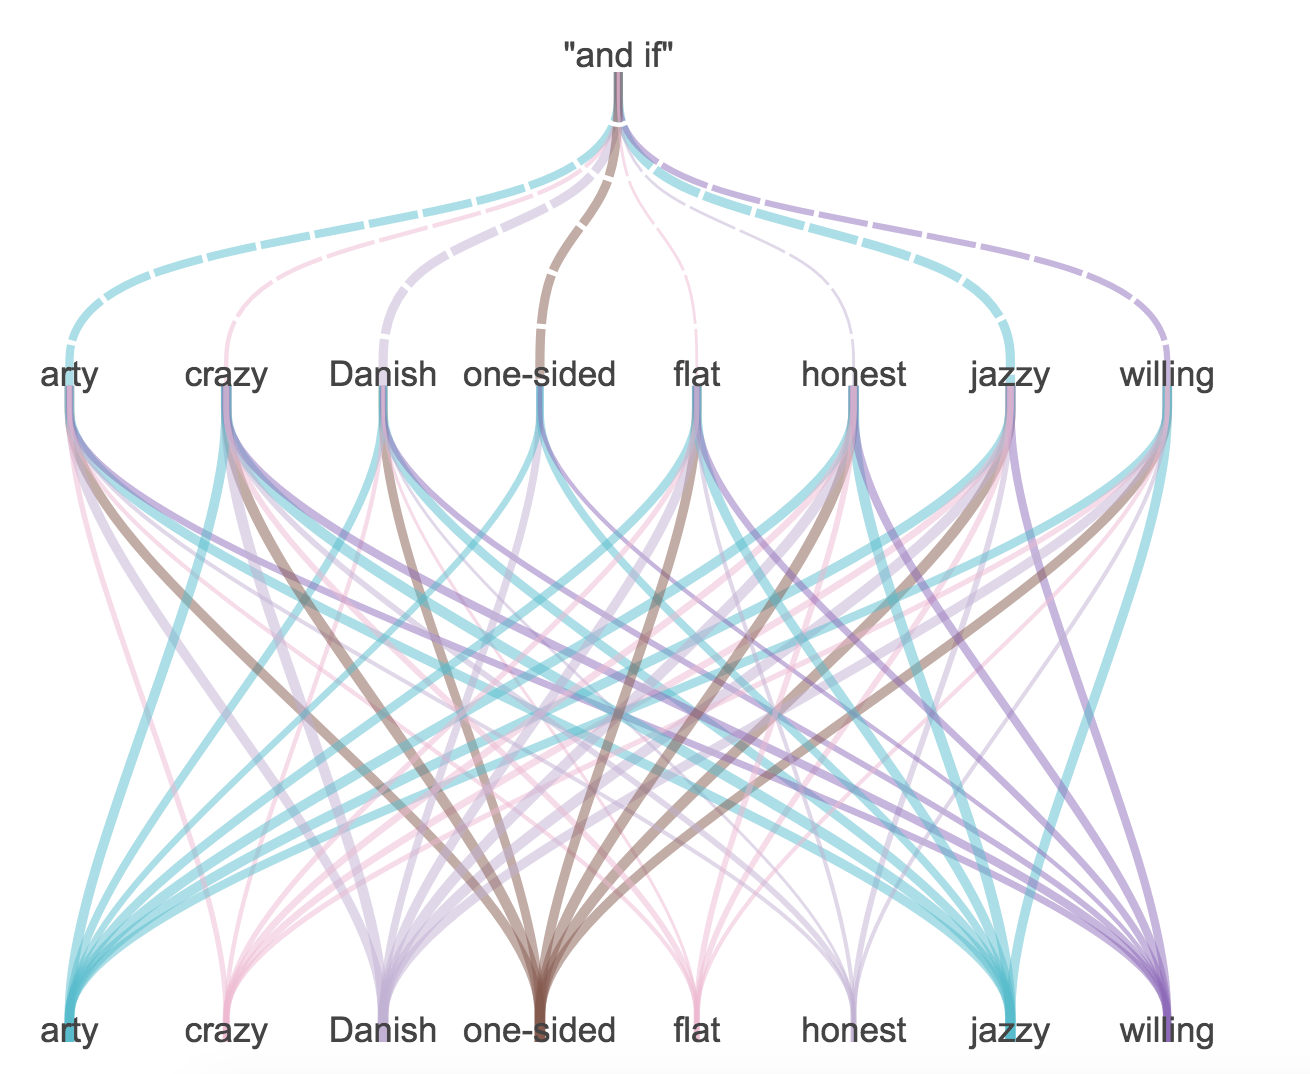
\includegraphics[width=7.5cm]{img/cooc_english2.png}
\caption{co-occurrences analysis of \textit{and if} showed by Hyperbase}
\label{and_if}
\end{center}
\end{figure}

In addition, we have the same behavior with the verb \textit{fall}. There is \textit{asleep} next to him. \textit{asleep} alone is not really specific of negative review (z-score of 1.13). But with the word \textit{fall}, \textit{asleep} become one of the most specific (see the co-occurrences analysis - Figure \ref{fall}).

\begin{figure}[h]
\begin{center}
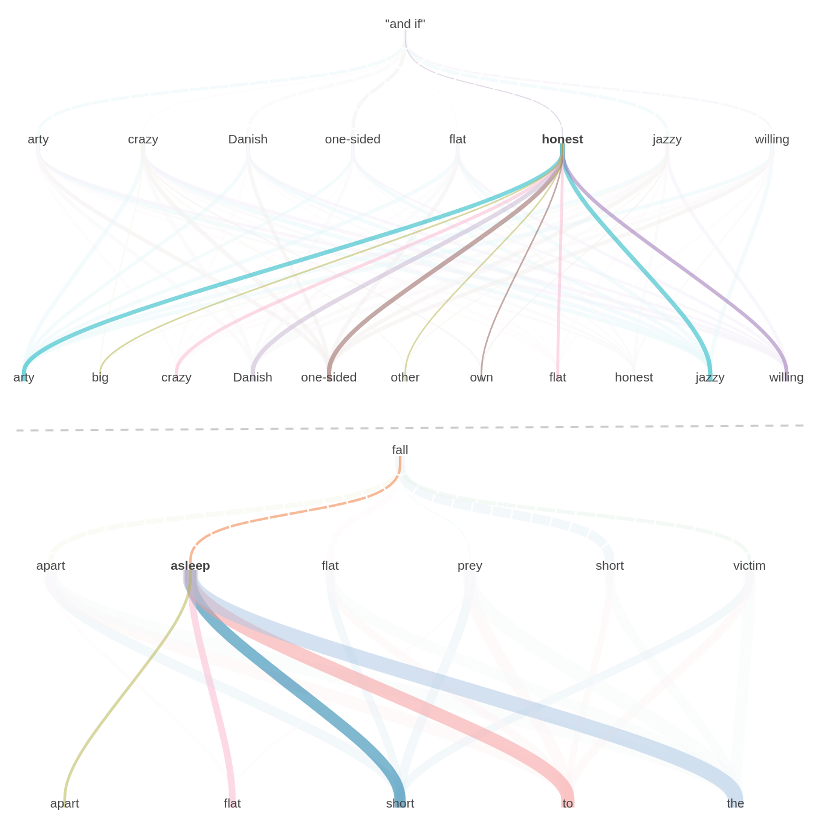
\includegraphics[width=7.5cm]{img/cooc_english.png}
\caption{co-occurrences analysis of \textit{fall} showed by Hyperbase}
\label{fall}
\end{center}
\end{figure}

The activation-score here confirms that deep learning seems to focus not only on high z-score but on more complex patterns and maybe detects the lemma or the part of speech linked to each word. While the embedding is modifiable during the learning, it's possible that the final word vectors share this kind of information. We will see now that these observations are still valid for other languages and can even be generalized between different activation spikes.

\subsection{Dataset: French}

The French data set consists of political speeches. It's a corpus of 2.5 millions of words of French Presidents from 1958 (with C. de Gaulle, the first President of the Fifth Republic) to 2018 with the first speeches by Macron. In this corpus we removed Macron's speech from the 31st of December 2017, to use it as a test data set. In this speech, the deeplearning network primarily recognizes E. Macron (the training task was to be able to predict the correct President). To achieve this task the deeplearning network seems to succeed in finding really complex patterns specific to E. Macron. For example in this sequence :

\begin{quote}
\textit{[...] notre pays \textcolor{red}{\textbf{advienne à}} l'école pour nos enfants, au travail pour l' ensemble de \textcolor{red}{\textbf{nos concitoyens}} pour le climat pour le quotidien de chacune et chacun d' entre vous . \textcolor{red}{\textbf{Ces transformations profondes}} ont commencé et se \textcolor{red}{\textbf{poursuivront}} avec la même force le même rythme la même intensité [...]} 
\end{quote}

\begin{figure}[h]
\begin{center}
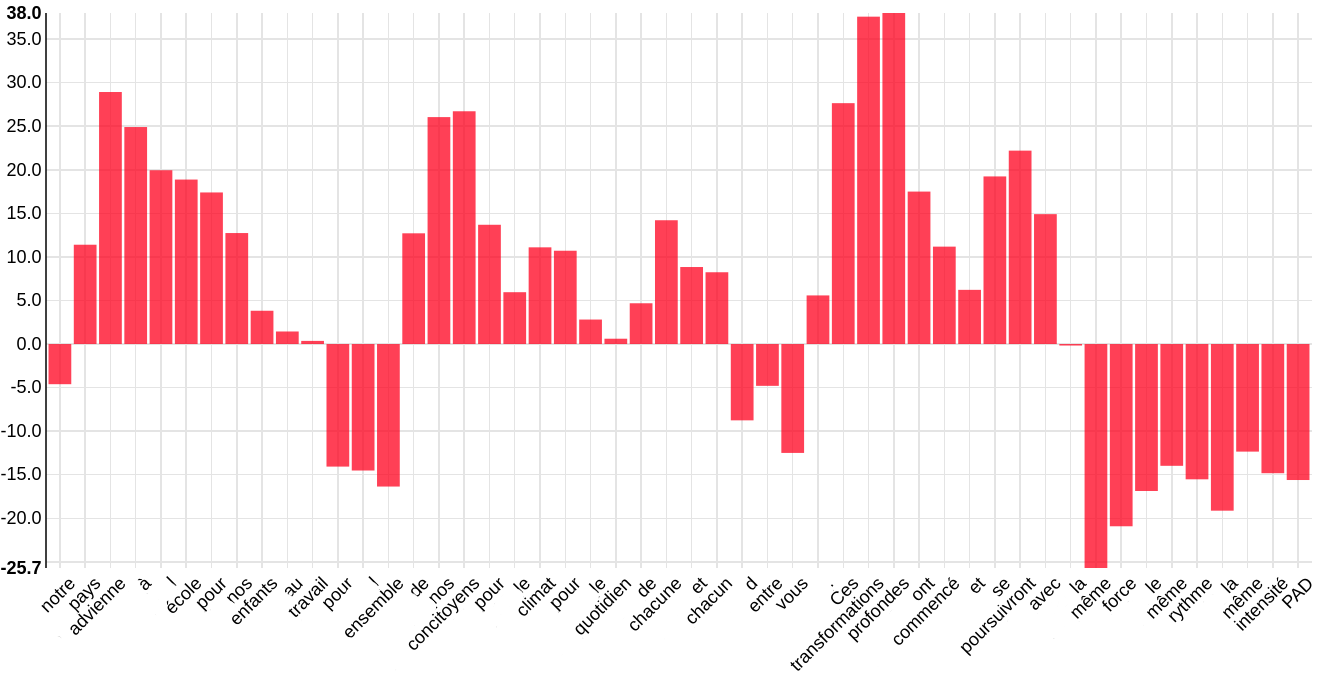
\includegraphics[width=7.5cm]{img/macron_activation.png}
\caption{Deconvolution on E. Macron speech.}
\label{macron_activation}
\end{center}
\end{figure}

The z-score gives a result statistically closer to De Gaulle than to E. Macron. The error in the statistical attribution can be explained by a Gaullist phraseology and the multiplication of linguistic markers strongly indexed with de Gaulle: for example, de Gaulle had the characteristic of making long and literary sentences articulated around conjunctions of coordination as in \textit{et} (z-score = 28 for de Gaulle, two occurrences in the excerpt). His speech was also more conceptual than average, and this resulted in an over-use of the articles defined \textit{le}, \textit{la}, \textit{l\'}, \textit{les}) very numerous in the excerpt(7 occurrences); especially in the feminine singular (\textit{la république}, \textit{la liberté}, \textit{la nation}, \textit{la guerre}, etc., here we have \textit{la même force}, \textit{la même intensité}.

The best results given by deeplearning themselves can surprise the linguist and match perfectly with what is known about the sociolinguistics of Macron's dynamic kind of speeches.

The most important activation zone of the excerpt concerns the nominal syntagm \textit{transformations profondes}. Taken separately, neither of the phrase's two words are very Macronian from a statistical point of view (\textit{transformations} = 1.9 \textit{profondes} = 2.9). Better: the syntagm itself is not attested in the President's learning corpus (0 occurrence). However, it can be seen that the co-occurrence of \textit{transformation} and \textit{profondes} amounts to 4.81 at Macron: so it is not the occurrence of one word alone, or the other, which is Macronian but the simultaneous appearance of both in the same window. The second and complementary activation zones of the excerpt thus concern the two verbs \textit{advienne} and \textit{poursuivront}. From a semantic point of view, the two verbs perfectly conspire, after the phrase \textit{transformations profondes}, to give the necessary dynamic to a discourse that advocates change. But it is the verb tenses (borne by the morphology of the verbs) that appear to be the determining factor in the analysis. The calculation of the grammatical codes co-occurring with the word \textit{transformations} thus indicates that the verbs in the subjunctive and the verbs in the future (and also the nouns) are the privileged codes for Macron (Figure \ref{macron}). 

\begin{figure}[h]
\begin{center}
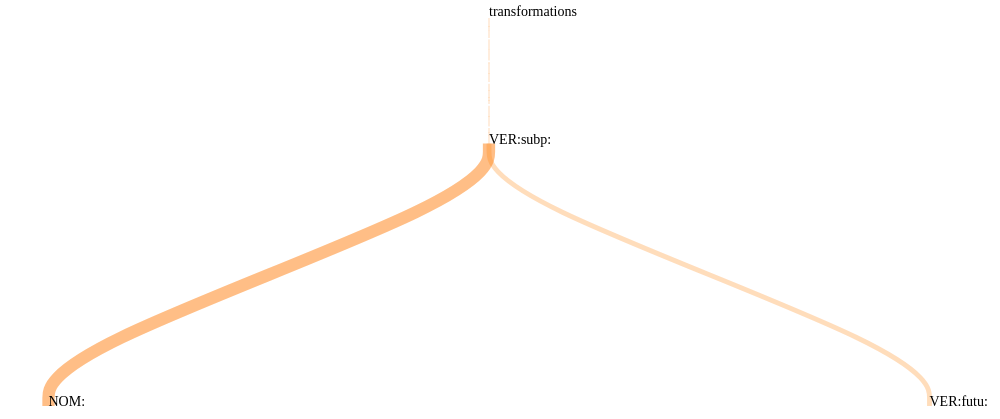
\includegraphics[width=7.5cm]{img/macron_cooc.png}
\caption{Main part-of-speech cooccurrences for \textit{transformations} showed by Hyperbase}
\label{macron}
\end{center}
\end{figure}


More precisely the algorithm indicates that, for Macron, when \textit{transformation} is associated with a verb in the subjunctive (here \textit{advienne}), then there is usually a verb in the future co-present (here \textit{poursuivront}). \textit{transformations profondes}, \textit{advienne} to the subjunctive, \textit{poursuivront} to the future: all these elements together form a speech promising action, from the mouth of a young and dynamic President. Finally, the graph indicates that \textit{transformations} is especially associated with nouns in the President's speeches: in an extraordinary concentration, the excerpt lists 11 (\textit{pays}, \textit{école}, \textit{enfants}, \textit{travail}, \textit{concitoyens}, \textit{climat}, \textit{quotidien}, \textit{transformations}, \textit{force}, \textit{rythme}, \textit{intensité}).

\subsection{Dataset: Latin}

The last dataset we used is based on Latin. We assembled a contrastive corpus of 2 million words with 22 principle authors writting in classical Latin. As in the French dataset, the learning task here was to be able to predict each author according to new sequences of words. The next example is a excerpt of chapter 26 of the 23th book of Livy:

\begin{quote}
\textit{[...] tutus tenebat se quoad multum ac diu PAD quattuor milia peditum et quingenti equites in supplementum missi ex PAD sunt . tum refecta tandem spe \textcolor{red}{\textbf{castra propius hostem}} mouit classem que et ipse instrui parari que iubet ad insulas maritimam que oram tutandam . in \textcolor{red}{\textbf{ipso impetu}} mouendarum de [...]} 
\end{quote}

The statistics here identify this sequence with Caesar\footnote{Gaius Julius Caesar, 100 BC - 44 BC, usually called Julius Caesar, was a Roman politician and general and a notable author of Latin prose.} but Livy is not far off. As historians, Caesar and Livy share a number of specific words: for example tool words like \textit{se} (reflexive pronoun) or \textit{que} (a coordinator) and prepositions like \textit{in}, \textit{ad}, \textit{ex}, \textit{of}. There are also names like \textit{equites} (cavalry) or \textit{castra} (fortified camp).

The attribution of the sentence to Caesar can not only rely only on z-score: \textit{que} or \textit{in} or \textit{castra}, with differences thereof equivalent or inferior to Livy. On the other hand, the differences of \textit{se}, \textit{ex}, are greater, as is that of \textit{equites}. Two very Caesarian terms undoubtedly make the difference \textit{iubet} (he orders) and \textit{milia} (thousands).

The greater score of \textit{quattuor} (four), \textit{castra}, \textit{hostem} (the enemy), \textit{impetu} (the assault) in Livy are not enough to switch the attribution to this author.

On the other hand, deeplearning activates several zones appearing at the beginning of sentences and corresponding to coherent syntactic structures (for Livy) -- \textit{Tandem reflexes spe castra propius hostem mouit} (then, hope having finally returned, he moved the camp closer to the camp of the enemy) -- despite the fact that \textit{castra} in \textit{hostem mouit} is attested only by Tacitus\footnote{Publius (or Gaius) Cornelius Tacitus, 56 BC - 120 BC, was a senator and a historian of the Roman Empire.}. 

There are also \textit{in ipso metu} (in fear itself), while \textit{in} followed by \textit{metu} is counted one time with Caesar and one time also with Quinte-Curce\footnote{Quintus Curtius Rufus was a Roman historian, probably of the 1st century, his only known and only surviving work being "Histories of Alexander the Great"}.

More complex structures are possibly also detected by deeplearning: the structure \textit{tum} + participates Ablative Absolute (\textit{tum refecta}) is more characteristic of Livy (z-score 3.3 with 8 occurrences) than of Caesar (z-score 1.7 with 3 occurrences), even if it is even more specific of Tacitus (z-score 4.2 with 10 occurrences).

Finally and more likely, the co-occurrence between \textit{castra}, \textit{hostem} and \textit{impetu} may have played a major role: Figure \ref{latin}

\begin{figure}[h]
\begin{center}
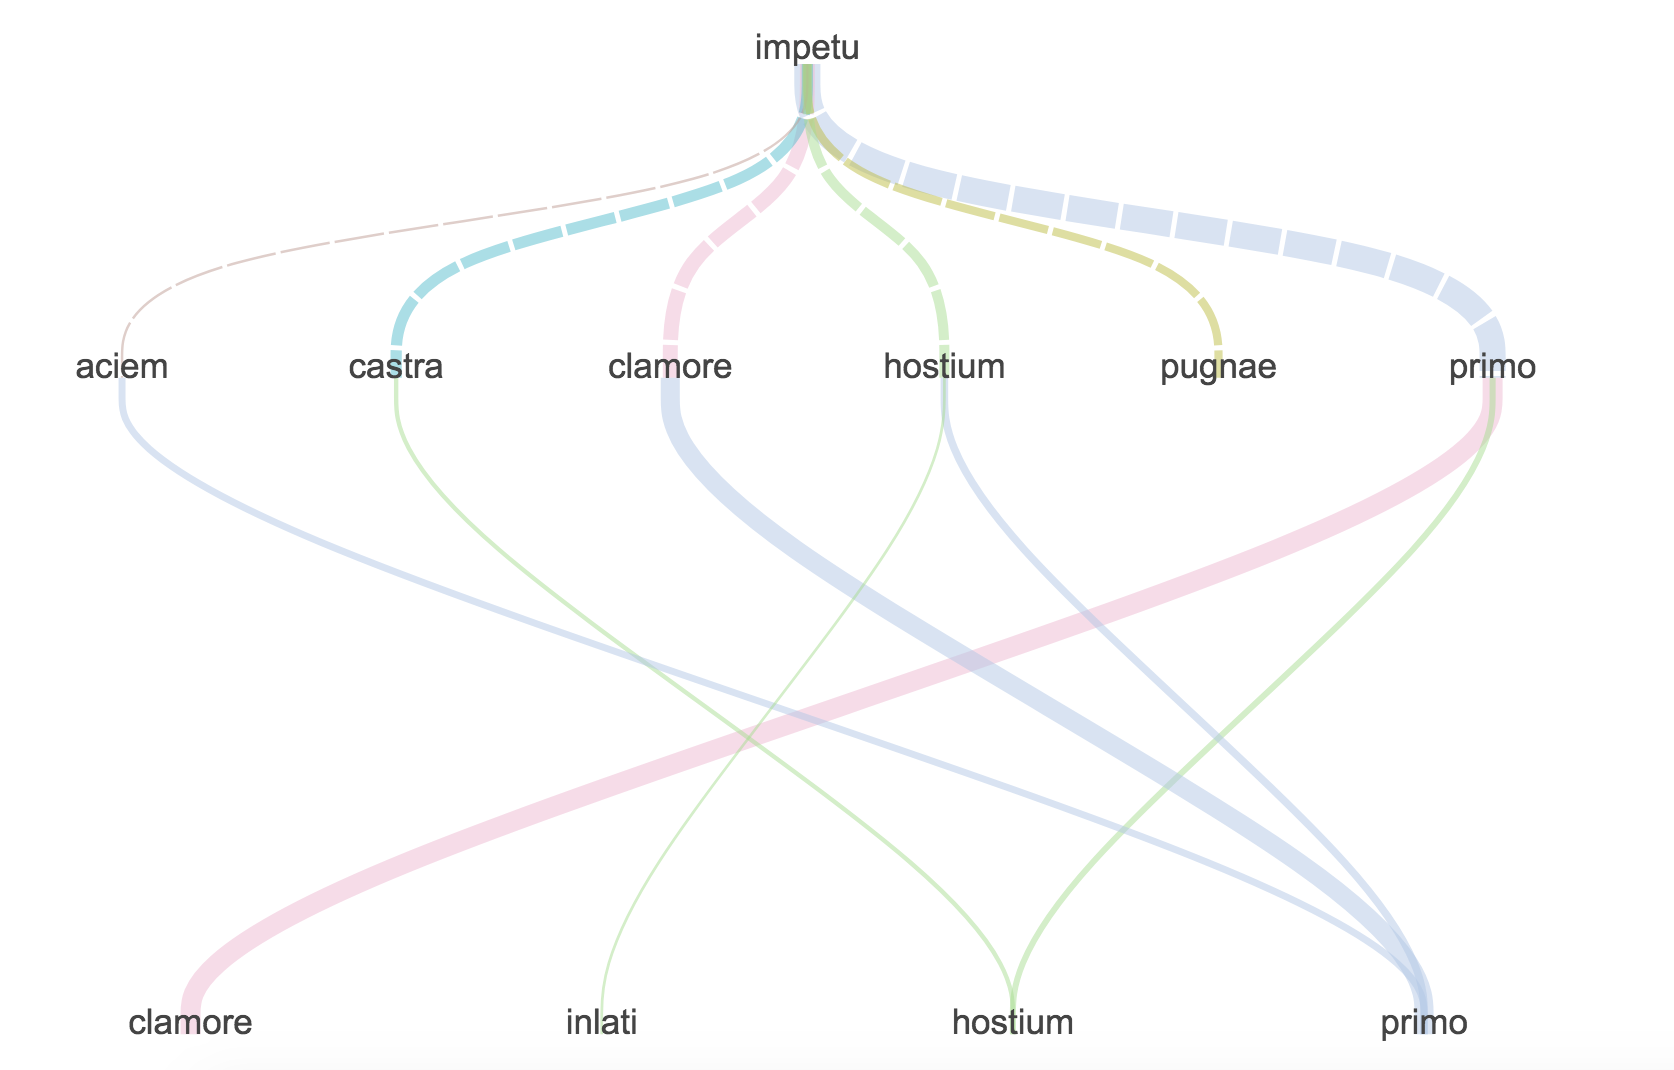
\includegraphics[width=7.5cm]{img/cooc_latin.png}
\caption{Specific co-occurrences between \textit{impetu} and \textit{castra} showed by Hyperbase.}
\label{latin}
\end{center}
\end{figure}

With Livy, \textit{impetu} appears as a co-occurrent with the lemmas \textit{HOSTIS} (z-score 9.42) and \textit{CASTRA} (z-score 6.75), while \textit{HOSTIS} only has a gap of 3.41 in Caesar and that \textit{CASTRA} does not appear in the list of co-occurrents.

For \textit{castra}, the first co-occurent for Livy is \textit{HOSTIS} (z-score 22.72), before \textit{CASTRA} (z-score 10.18), \textit{AD} (z-score 10.85), \textit{IN} (z-score 8.21), \textit{IMPETVS} (z-score 7.35), \textit{QUE} (z-score 5.86) ) while in Caesar, \textit{IMPETVS} does not appear and the scores of all other lemmas are lower except \textit{CASTRA} (z-score 15.15), \textit{HOSTIS} (8),  \textit{AD} (10,35), \textit{IN} (5,17), \textit{QUE} (4.79).

Thus, all is as it should be if the deeplearning network manages to simultaniously account for specificity, phrase structure, and co-occurence networks\ldots


